
\documentclass[]{article}
\voffset=-1.5cm
\oddsidemargin=0.0cm
\textwidth = 480pt


\usepackage{amsmath}
\usepackage{graphicx}
\usepackage{amssymb}
\usepackage{framed}
\usepackage{multicol}
%\usepackage[paperwidth=21cm, paperheight=29.8cm]{geometry}
%\usepackage[angle=0,scale=1,color=black,hshift=-0.4cm,vshift=15cm]{background}
%\usepackage{multirow}
\usepackage{enumerate}






\begin{document}
%%- http://www.maths-statistics-tutor.com/normality_test_pasw_spss.php
%%- http://webspace.ship.edu/pgmarr/Geo441/Lectures/Lec%205%20-%20Normality%20Testing.pdf

\section{Testing for Normality using SPSS Statistics}

\subsection{Introduction}
An assessment of the normality of data is a prerequisite for many statistical tests because normal data is an underlying assumption in parametric testing. There are two main methods of assessing normality: graphically and numerically.
%===============================================================%
This "quick start" guide will help you to determine whether your data is normal, and therefore, that this assumption is met in your data for statistical tests. The approaches can be divided into two main themes: relying on statistical tests or visual inspection. Statistical tests have the advantage of making an objective judgement of normality, but are disadvantaged by sometimes not being sensitive enough at low sample sizes or overly sensitive to large sample sizes. 
%===============================================================%
\begin{itemize}
\item As such, some statisticians prefer to use their experience to make a subjective judgement about the data from plots/graphs. 
\item Graphical interpretation has the advantage of allowing good judgement to assess normality in situations when numerical tests might be over or under sensitive, but graphical methods do lack objectivity. 
\item If you do not have a great deal of experience interpreting normality graphically, it is probably best to rely on the numerical methods.
%===============================================================%
%%\item If you want to be guided through the testing for normality procedure in SPSS Statistics for the specific statistical test you are using to analyse your data, we provide comprehensive guides in our enhanced content.
\item  For each statistical test where you need to test for normality, we show you, step-by-step, the procedure in SPSS Statistics, as well as how to deal with situations where your data fails the assumption of normality (e.g., where you can try to "transform" your data to make it "normal"; something we also show you how to do using SPSS Statistics). 
%% \item You can learn about our enhanced content in general here or how we help with assumptions here. However, in this "quick start" guide, we take you through the basics of testing for normality in SPSS Statistics.
\end{itemize}
%===============================================================%
\subsection{Methods of assessing normality}
\begin{itemize}
	\item SPSS Statistics allows you to test all of these procedures within \texttt{Explore...} command. 
	\item The \texttt{Explore...} command can be used in isolation if you are testing normality in one group or splitting your dataset into one or more groups. 
	\item For example, if you have a group of participants and you need to know if their height is normally distributed, everything can be done within the \texttt{Explore...} command. 
	\item If you split your group into males and females (i.e., you have a categorical independent variable), you can test for normality of height within both the male group and the female group using just the \texttt{Explore...} command. 
	\item This applies even if you have more than two groups. 
	\item However, if you have 2 or more categorical, independent variables, the \texttt{Explore...} command on its own is not enough and you will have to use the Split File... command also.
	
\end{itemize}


%===============================================================%

\subsection{Procedure for none or one grouping variable}
The following example comes from our guide on how to perform a one-way ANOVA in SPSS Statistics.

Click Analyze > Descriptive Statistics > Explore... on the top menu, as shown below:

\begin{figure}
\centering
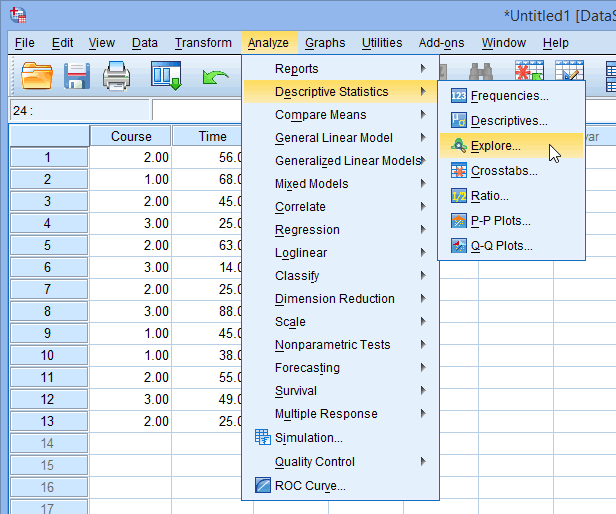
\includegraphics[width=0.7\linewidth]{Normality/normality-1}
\caption{}
\label{fig:normality-1}
\end{figure}

%===============================================================%
You will be presented with the Explore dialogue box, as shown below:

\begin{figure}
	\centering
	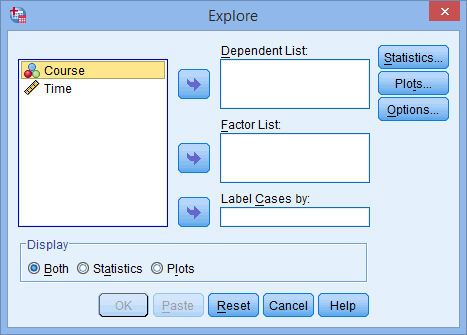
\includegraphics[width=0.7\linewidth]{Normality/normality-2}
	\caption{}
	\label{fig:normality-2}
\end{figure}
%===============================================================%
Transfer the variable that needs to be tested for normality into the Dependent List: box by either drag-and-dropping or using the SPSS Arrow Right Button button. In this example, we transfer the Time variable into the Dependent List: box. You will then be presented with the following screen:

\begin{figure}
	\centering
	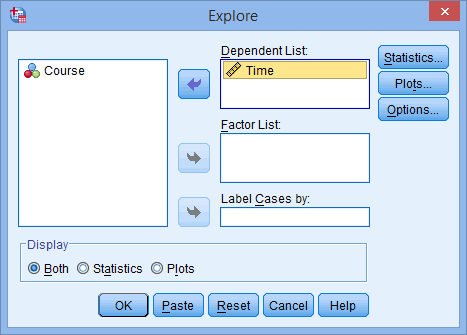
\includegraphics[width=0.7\linewidth]{Normality/normality-3}
	\caption{}
	\label{fig:normality-3}
\end{figure}
%===============================================================%
[Optional] If you need to establish if your variable is normally distributed for each level of your independent variable, you need to add your independent variable to the Factor List: box by either drag-and-dropping or using the SPSS Arrow Right Button button. In this example, we transfer the Course variable into the Factor List: box. You will be presented with the following screen:

\begin{figure}
	\centering
	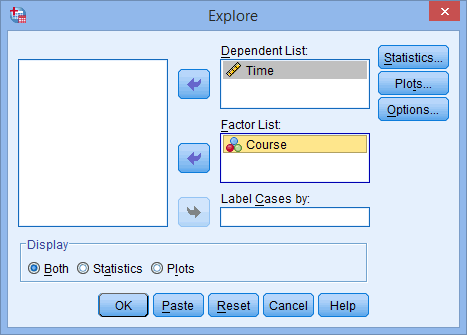
\includegraphics[width=0.7\linewidth]{Normality/normality-4}
	\caption{}
	\label{fig:normality-4}
\end{figure}
%===============================================================%
Click the SPSS Statistics Button button. You will be presented with the Explore: Statistics dialogue box, as shown below:

\begin{figure}
	\centering
	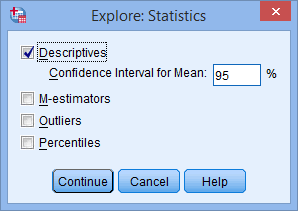
\includegraphics[width=0.7\linewidth]{Normality/normality-5}
	\caption{}
	\label{fig:normality-5}
\end{figure}
%===============================================================%
Leave the above options unchanged and click the SPSS Continue Button button.

Click the SPSS Plots Button button. Change the options so that you are presented with the following screen:


\begin{figure}
	\centering
	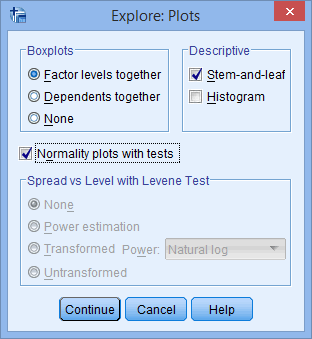
\includegraphics[width=0.7\linewidth]{Normality/normality-6}
	\caption{}
	\label{fig:normality-6}
\end{figure}

%===============================================================%
Click the  button.

Click the  button.

%==================================================================================%
\subsection{Output}
SPSS Statistics outputs many table and graphs with this procedure. One of the reasons for this is that the \texttt{Explore...} command is not used solely for the testing of normality, but in describing data in many different ways. When testing for normality, we are mainly interested in the Tests of Normality table and the Normal Q-Q Plots, our numerical and graphical methods to test for the normality of data, respectively.

\subsection{Shapiro-Wilk Test of Normality}

\begin{figure}
	\centering
	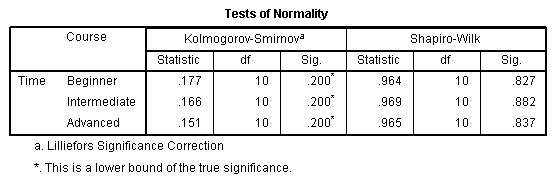
\includegraphics[width=0.7\linewidth]{Normality/normality-7}
	\caption{}
	\label{fig:normality-7}
\end{figure}
%===============================================================%
\begin{itemize}
	\item The above table presents the results from two well-known tests of normality, namely the Kolmogorov-Smirnov Test and the Shapiro-Wilk Test. The Shapiro-Wilk Test is more appropriate for small sample sizes (< 50 samples), but can also handle sample sizes as large as 2000. For this reason, we will use the Shapiro-Wilk test as our numerical means of assessing normality.
	
\item We can see from the above table that for the "Beginner", "Intermediate" and "Advanced" Course Group the dependent variable, "Time", was normally distributed.
\item \textbf{IMPORTANT }How do we know this? If the Sig. value of the Shapiro-Wilk Test is greater than 0.05, the data is normal. If it is below 0.05, the data significantly deviate from a normal distribution.
	
%\item If you need to use skewness and kurtosis values to determine normality, rather the Shapiro-Wilk test, you will find these in our enhanced testing for normality guide. You can learn more about our enhanced content here.
\end{itemize}


%===============================================================%
\subsection{Normal Q-Q Plot}
\begin{itemize}
	\item In order to determine normality graphically, we can use the output of a normal Q-Q Plot. If the data are normally distributed, the data points will be close to the diagonal line. 
	\item If the data points stray from the line in an obvious non-linear fashion, the data are not normally distributed. 
	\item As we can see from the normal Q-Q plot below, the data is normally distributed. 
	\item If you are at all unsure of being able to correctly interpret the graph, rely on the numerical methods instead because it can take a fair bit of experience to correctly judge the normality of data based on plots.
\end{itemize}


Normality Screenshot
%===============================================================%
If you need to know what Normal Q-Q Plots look like when distributions are not normal (e.g., negatively skewed), you will find these in our enhanced testing for normality guide. You can learn more about our enhanced content here.


%===============================================================%

%%Testing for Normality using SPSS Statistics (cont...)
\newpage
\section{Procedure when there are two or more independent variables}
The Explore... command on its own cannot separate the dependent variable into groups based on not one but two or more independent variables. However, we can perform this feat by using the Split File... command.

Click Data > Split File... on the top menu as shown below:

\begin{figure}
	\centering
	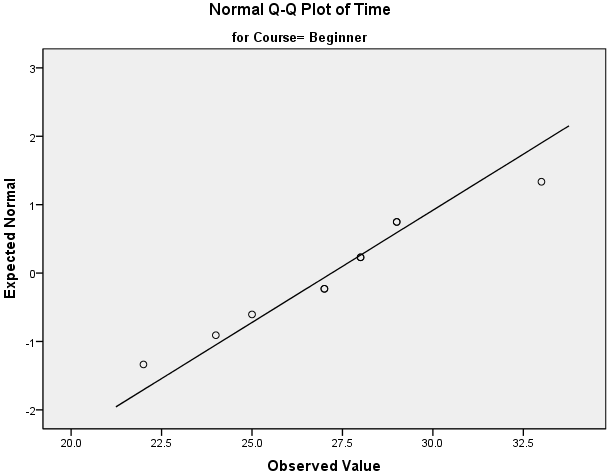
\includegraphics[width=0.7\linewidth]{Normality/normality-8}
	\caption{}
	\label{fig:normality-8}
\end{figure}
%===============================================================%
You will be presented with the Split File dialogue box, as shown below:

Normality Screenshot
%===============================================================%
\begin{itemize}
	\item Click the radio option, Organize output by groups. Transfer the independent variables you wish to categorize the dependent variable on into the Groups Based on: box. 
	\item In this example, we want to know whether interest in politics (Int\_Politics) is normally distributed when grouped/categorized by Gender AND Edu\_Level (education level). You will be presented with the following screen:
\end{itemize}


Normality Screenshot

%===============================================================%
Click the SPSS OK Button button.

Note: Your file is now split and the output from any tests will be organized into the groups you have selected.

Click Analyze > Descriptive Statistics > Explore... on the top menu as shown below:

Normality Screenshot

%===============================================================%
You will be presented with the Explore dialogue box, as shown below:

Normality Screenshot
%===============================================================%
Leave the above options unchanged and click the SPSS Continue Button button.

\begin{itemize}
	\item Transfer the variable that needs to be tested for normality into the Dependent List: box by either drag-and-dropping or using the SPSS Right Arrow Button button. In this example, we transfer the \texttt{Int\_Politics} variable into the Dependent List: box. You will then be presented with the following screen:
\end{itemize}


Normality Screenshot
Published with written permission from SPSS Statistics, IBM Corporation.

\begin{framed}
Note: There is no need to transfer the independent variables \texttt{Gender} and \texttt{Edu\_Level} into the Factor List: box because this has been accomplished with the Split File... command. We cannot simply transfer these two independent variables into the Factor List: box because this will not achieve the desired result. It will first analyse \texttt{Int\_Politics} for normality with respect to Gender and then with respect to \texttt{Edu\_Level}. It does NOT analyse \texttt{Int\_Politics} for normality by grouping individuals into both Gender and \texttt{Edu\_Level} AT THE SAME TIME.
\end{framed}

%===============================================================%
Click the SPSS Statistics Button button. You will be presented with the Explore: Statistics dialogue box, as shown below:

Normality Screenshot

%===============================================================%
Leave the above options unchanged and click the SPSS Continue Button button.

Click the SPSS Plots Button button. Change the options so that you are presented with the following screen:

Normality Screenshot
%===============================================================%
Click the  button.

Click the  button.

%================================================================%
\section{Output}
You will now see that the output has been split into separate sections based on the combination of groups of the two independent variables. As an example we show the tests of normality when the dependent variable, "\texttt{Int\_Politics}", is categorized into the first "Gender" group (male) and first "\texttt{Edu\_Level}" group (School). All other possible combinations are also presented in the full output but we will not shown them here for clarity.

Normality Screenshot

%===============================================================%
Under this above category you are presented with the Tests of Normality table as shown below:

Normality Screenshot
Published with written permission from SPSS Statistics, IBM Corporation.

\begin{itemize}
	\item The Shapiro-Wilk test is now analysing the normality of "\texttt{Int\_Politics}" on the data of those individuals that are classified as both "male" in the independent variable, "Gender", and "school" in the independent variable "\texttt{Edu\_Level}". As the Sig. value under the Shapiro-Wilk column is greater than 0.05, we can conclude that "\texttt{Int\_Politics}" for this particular subset of individuals is normally distributed.

%===============================================================%
	\item  The same data from the same individuals are now also being analysed to produce a Normal Q-Q Plot as below. From this graph, we can conclude that the data appears to be normally distributed as it follows the diagonal line closely and does not appear to have a non-linear pattern.
\end{itemize}



Normality Screenshot

%===============================================================%
\end{document}
